\documentclass[10pt,letterpaper]{article}

\usepackage[utf8]{inputenc}
\usepackage[spanish,es-nodecimaldot]{babel}
\usepackage{amsmath}
\usepackage{amssymb}
\usepackage{graphicx}
\usepackage{mathtools}

\usepackage{multicol}

\usepackage{enumitem}

\newcommand{\ihat}{\hat{\textbf{\i}}}
\newcommand{\jhat}{\hat{\textbf{\j}}}
\newcommand{\uhat}{\hat{\textbf{u}}}
\DeclarePairedDelimiter{\norm}{\lVert}{\rVert}

\usepackage[top=1in, bottom=1in, left=1in, right=1in]{geometry}


\begin{document}

\begin{titlepage}
    \centering

    {\scshape\LARGE Universidad Nacional Autónoma de México \par}

    \vspace{1cm}
    {\scshape\Large Facultad de Ciencias\par}
    \vspace{1.5cm}

    \begin{center}
        
\includegraphics[scale=.1]{../../assets/img/logo.png}
    \end{center}

    \vspace{.8 cm}

    {\LARGE Tarea 02: \par}
    {\huge\bfseries Convexidad, vecindarios, búsqueda local: Hill Climbing y Búsqueda Tabú \par}

    \vspace{0.5cm}
    \large{\itshape{Pablo A. Trinidad Paz}} \small{ - 419004279}

    \vfill

    Trabajo presentado como parte del curso de
    \textbf{Cómputo Evolutivo}
    impartido por el profesor \textbf{Mario Iván Jaen Márquez}. \par
    \vspace{0.5cm}
    Fecha de entrega: \textbf{22 de Febrero de 2019}.
\end{titlepage}

\section{Teoría}
    \begin{enumerate}
        \item Sean $f_2, f_2: \mathbb{R} \rightarrow \mathbb{R}$ dadas por
            \begin{equation*} \begin{split} \begin{aligned}
                f_1(x) &= x^2 - 2ex + e^2 - 2, \\
                f_2(x) &= x^6 - 6ex^5 + 15e^2x^4 - 20e^3x^3 + 15e^4x^2 - 6e^5x + e^6 - 6 \\
            \end{aligned} \end{split} \end{equation*} \\

            \begin{enumerate}
                \item Demuestre que $f_1$ y $f_2$ son funciones convexas \\

                    \textbf{Solución:}

                    Una función $f$ es convexa si se cumple que:
                    \begin{equation*} \begin{split} \begin{gathered}
                        \forall x, y \in Dom(f)  \text{ y } \forall a \in [0, 1] \\
                        f(ax + (1-a)y) \leq af(x) + (1 - a)f(y).
                    \end{gathered} \end{split} \end{equation*}
                    Además, se cumple que si la función es doblemente derivable
                    (y de una sola variable) es convexa en un intervalo sí y solo sí
                    su segunda derivada no es negativa.

                    Para $f_1(x)$:
                    \begin{equation*} \begin{split} \begin{gathered}
                        f_1'(x) = 2x - 2e \\
                        f_1''(x) = 2 \\
                        \Rightarrow f_1''(x) > 0 \\
                        \therefore \; f_1 \text{ es convexa} \quad \blacksquare
                    \end{gathered} \end{split} \end{equation*}

                    Para $f_2(x)$:
                    \begin{equation*} \begin{split} \begin{gathered}
                        f_2'(x) =  6 x^5  - 30 e x^4  + 60 e^2 x^3  - 60 e^3 x^2 + 30 e^4 x - 6 e^5  \\
                        f_2''(x) = 30 x^4 - 120 e x^3 + 180 e^2 x^2 - 120 e^3 x  + 30 e^4 \\
                        f_2''(x) = 30(e - x)^4 \\
                        \Rightarrow f_2''(x) > 0 \\
                        \therefore \; f_2 \text{ es convexa} \quad \blacksquare
                    \end{gathered} \end{split} \end{equation*}

                \item Utilice el algoritmo del descenso por gradiente implementado
                para minimizarlas. Use $x_0 = 0$ como punto inicial y $\alpha$
                arbitrario. ¿Qué valores de $\alpha$ hacen más eficiente el algoritmo
                para cada función? \\

                    \textbf{Solución:} \\
                    Para responder a la pregunta anterior se corrió el
                    descenso por gradiente con múltiples valores de $\alpha$
                    y se determinó que el valor de $\alpha$ más eficiente sería
                    aquel que lograra encontrar un óptimo en el menor número
                    de iteraciones. Para saber si el valor óptimo obtenido
                    a partir de dicha $\alpha$ era aceptable, se calculó la
                    desviación estándar, promedio y media de los resultados
                    de cada prueba. \\

                    Para ambas funciones, el gradiente corrió bajo los
                    siguientes parámetros:

                        \begin{itemize}
                            \item Precisión: $1 \times 10^{-8}$
                            \item Número máximo de iteraciones: $10^6$
                        \end{itemize}

                    \clearpage

                    \textbf{Resultados de $f_1$}: \\

                    \begin{center}
                        Valores de $\alpha$ para la función $f_1$ \\
                        \begin{tabular}{c|r|l} 
                            \hline
                            \multicolumn{1}{|c|}
                            {$\alpha$} & \textbf{Número de iteraciones} & \multicolumn{1}{l|}{\textbf{Valor mínimo}}  \\ 
                            \hline
                            0.000005    &   790773  &   2.7172818427188603  \\
                            0.00001     &   430042  &   2.7177818402339007   \\
                            0.00005     &   102100  &   2.7181818454738185  \\
                            0.0001      &   54513   &   2.718231838600649 \\
                            0.0005      &   12508   &   2.7182718417772485 \\
                            0.001       &   6598    &   2.7182768441392824 \\
                            0.005       &   1476    &   2.7182808470688657 \\
                            0.01        &   769     &   2.71828134188752 \\
                            0.05        &   164     &   2.7182817433322994 \\
                            0.1         &   81      &   2.718281790036739 \\
                            0.5         &   2       &   2.718281828459045
                        \end{tabular}
                    \end{center}

                    \begin{multicols}{2}
                        \begin{center}
                            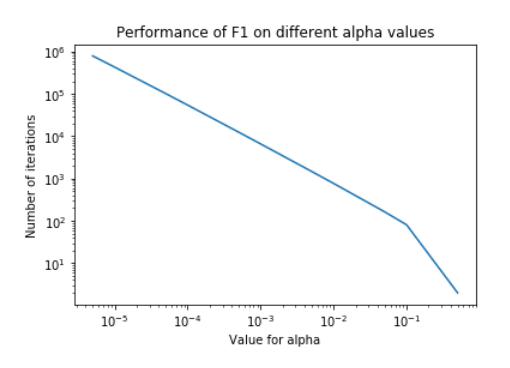
\includegraphics[scale=.4]{assets/theory/1-a/f1-performance.png}
                        \end{center}
                        \begin{center}
                            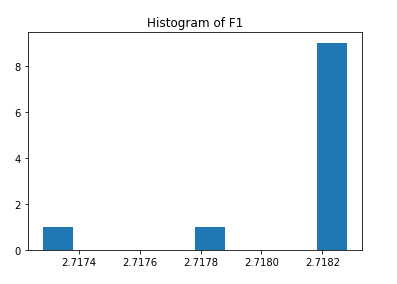
\includegraphics[scale=.5]{assets/theory/1-a/f1-dist.png}
                        \end{center}
                    \end{multicols}

                    Con una desviación estándar $\sigma \approx .000303$,
                    promedio $\mu \approx 2.7181303276$ y media $\approx 2.7182768441$
                    se puede concluir de forma segura que el valor óptimo de $\alpha$ para
                    $f_1$ es \textbf{0.5} y que el mínimo se encuentra en
                    $x=2.718281828459045$.

                    \begin{center}
                        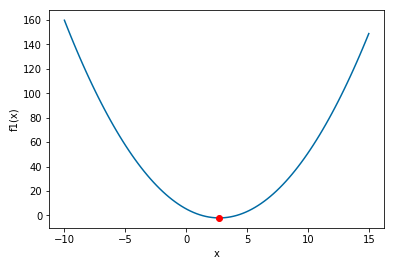
\includegraphics[scale=.5]{assets/theory/1-a/f1-minimum.png}
                    \end{center}

                    \clearpage

                    \textbf{Resultados de $f_2$}: \\
                    \begin{center}
                    Valores de $\alpha$ para la función $f_2$ \\
                    \begin{tabular}{c|r|l} 
                        \hline
                        \multicolumn{1}{|c|}
                        {$\alpha$} & \textbf{Número de iteraciones} & \multicolumn{1}{l|}{\textbf{Valor mínimo}}  \\ 
                        \hline
                            0.000005   &   1000000     &   2.3511877960913052 \\
                            0.00001   &   1000000     &   2.398706503240198 \\
                            0.00005   &   1000000     &   2.4866593461920012 \\
                            0.0001  &   1000000     &   2.51664267509827 \\
                            0.0005  &   1000000     &   2.57213799938737 \\
                            0.001   &   1000000     &   2.591415514678928

                        \end{tabular}
                    \end{center}
            \end{enumerate}
    \end{enumerate}

\section{Práctica}

\end{document}
